\documentclass{beamer}

% Russian-specific packages
\usepackage[T2A]{fontenc} % поддержка специальных русских символов
\usepackage[english,russian]{babel}
\usepackage[utf8]{inputenc}

% русские переносы
\usepackage{hyphenat}
% \hyphenation{ма-те-ма-ти-ка вос-ста-нав-ли-вать}

% путь к папке с изображениями
\graphicspath{{./figs/}}

% выравнивание по центру подписей к картинкам
\usepackage[justification=centering]{caption}

% Стиль презентации
\usetheme{Warsaw}
\usecolortheme{crane}
% Стиль цитирования
\bibliographystyle{utf8gost71u}

\usepackage{IEEEtrantools} % для создания многострочных математических формул
\usepackage{amsmath} % для математических формул и для автоматического добавления скобок при цитировании
\usepackage{commath} % для знака модуля

% Переопределение настроек цитирование на схожие с article
\usepackage[numbers]{natbib}
% make bibliography entries smaller
\renewcommand\bibfont{\scriptsize}
% If you have more than one page of references, you want to tell beamer
% to put the continuation section label from the second slide onwards
\setbeamertemplate{frametitle continuation}[from second]
% Now get rid of all the colours
\setbeamercolor*{bibliography entry title}{fg=black}
\setbeamercolor*{bibliography entry author}{fg=black}
\setbeamercolor*{bibliography entry location}{fg=black}
\setbeamercolor*{bibliography entry note}{fg=black}
% and kill the abominable icon
\setbeamertemplate{bibliography item}{}

% Замена стандартного (Cont.) на русский язык
\setbeamertemplate{frametitle continuation}[from second][(продолжение)]

% Убрать из подписи картинки префикс Рис.
\usepackage{caption}
\captionsetup[figure]{labelformat=empty}

% Убрать управляющие значки внизу слайдов
\beamertemplatenavigationsymbolsempty

% Переопределение нижней статусной строки,
% используется здесь для комбинации автора, института, темы и номера слайда
\setbeamertemplate{footline}{
\leavevmode%
\hbox{%
\begin{beamercolorbox}[wd=.5\paperwidth,ht=2.25ex,dp=1ex,center]{author in head/foot}%
    \usebeamerfont{title in head/foot}\insertshortauthor \hspace*{1em} (\insertshortinstitute)
\end{beamercolorbox}%
\begin{beamercolorbox}[wd=.4\paperwidth,ht=2.25ex,dp=1ex,center]{title in head/foot}%
    \usebeamerfont{title in head/foot}\insertshorttitle
\end{beamercolorbox}%
\begin{beamercolorbox}[wd=.1\paperwidth,ht=2.25ex,dp=1ex,center]{author in head/foot}%
    \insertframenumber{} / \inserttotalframenumber 
\end{beamercolorbox}}%
\vskip0pt%
}

\begin{document}

% Оформление титульного листа
\title[Развитие ППРЭ]
{Развитие метода разностной эволюции
для поиска параметров математических моделей}
\author[Свичкарев Анатолий]
{Студент: \textbf{Свичкарев Анатолий, группа 53601/4}\\
Научный руководитель: \textbf{Козлов Константин Николаевич}}
\institute[СПбПУ]
{Санкт-Петербургский Государственный
Политехнический Университет\\Петра Великого}
\date{март, 2016}

% Создание заглавной страницы
\frame{\titlepage} 

\begin{frame}{Введение}
    Проведение вычислительного эксперимента
    с помощью \textbf{математической модели}
    в большинстве случаев обходится \textbf{значительно дешевле},
    чем проведение соответствующего эксперимента
    над реальным биологическим объектом,
    кроме того \textbf{некоторые условия
    невозможно воспроизвести в лаборатории}.
    \bigskip

    Математические модели в биоинформатике в
    большинстве случаев создаются в таких компьютерных
    системах расчетов как \textbf{R, Python, Octave} и др.
    \bigskip

    Нахождение параметров в таких моделях требует
    многократного вычисления решений, что влечет
    \textbf{большие накладные расходы} на запуск того или иного
    интерпретатора.
\end{frame}

\begin{frame}{Цель}
    Целью работы является
    \textbf{развитие метода ППРЭ},
    а именно, разработка механизма
    асинхронного взаимодействия метода
    и минимизируемой функции отклонения
    решения математической модели от данных.

    \bigskip
    За счет единовременной загрузки
    неизменяемых данных и
    асинхронной загрузки переменных параметров
    планируется достигнуть
    \textbf{сокращения времени вычисления}
    при использовании
    интерпретируемых языков, например,
    для системы статистических расчетов R.
\end{frame}

\begin{frame}{Задачи}
\begin{enumerate}
    \itemsep 2em
    \item реализовать расширение программы ППРЭ,
        позволяющее запускать нужное количество копий
        интерпретатора один раз при старте.
    \item провести численные эксперименты с тестовыми функциями
    \item провести сравнительный анализ полученных результатов
\end{enumerate}
\end{frame}

\begin{frame}{Разностная эволюция}
    \begin{block}{Разностная эволюция}
        --- стохастический итерационный алгоритм минимизации,
        предложенный Сторном и Прайсом в 1995 г.
    \end{block}
    \begin{figure}[!h]
        \centering
        % TODO максимальный доступный размер
        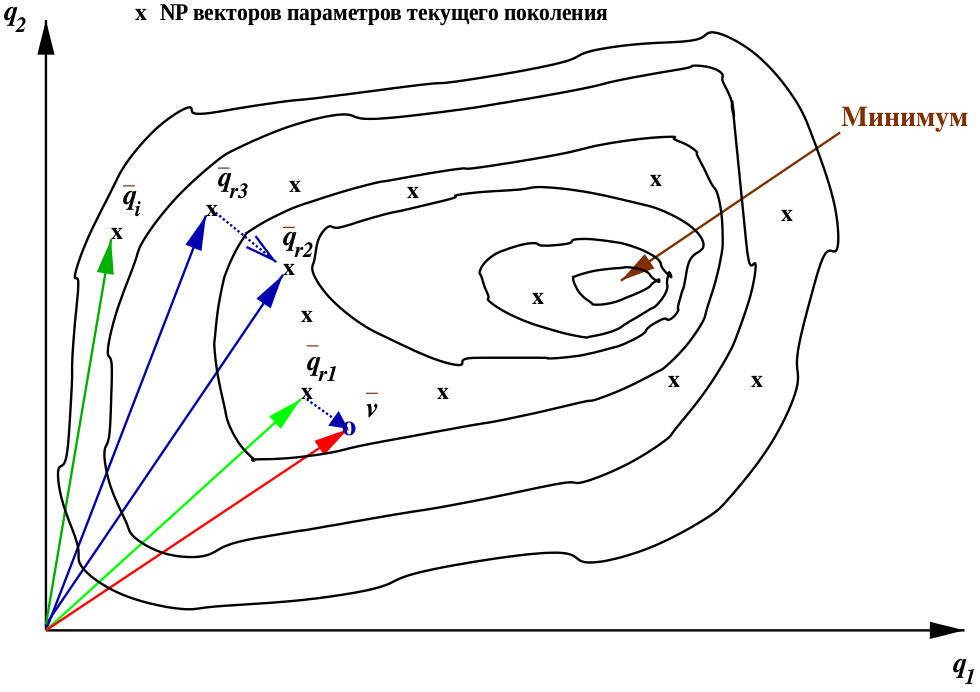
\includegraphics[scale=0.2]{DE}
        \caption{Геометрическая интерпретация метода разностной эволюции}
    \end{figure}
\end{frame}

\begin{frame}{Полностью параллельная разностная эволюция}
    \begin{block}{Полностью параллельная разностная эволюция (ППРЭ, DEEP)}
        --- эффективный метод решения
        обратной задачи математического моделирования,
        модификация глобального стохастического метода.
    \end{block}
    \bigskip

    Модификации разностной эволюции,
    реализованные в DEEP:
    \bigskip

    \begin{itemize}
        \itemsep 1em
        \item Скрещивание с учётом значения функционала;
        \item Скрещивание для поддержания разнообразия индивидов.
        \item Учёт возраста индивида в ходе эволюции.
    \end{itemize}
\end{frame}

\begin{frame}{Улучшение взаимодействия. Суть задачи.}
    \large{\textbf{Старая реализация:}}\\
    Для вычисления функционала
    качества каждый раз запускался
    новый экземпляр интерпретатора.
    \bigskip

    \large{\textbf{Новая реализация:}}\\
    Создаётся \textbf{пул потоков},
    где в каждом потоке запускается интерпретатор
    и инициализируется функцией из скрипта.\\
    Создаётся \textbf{асинхронная очередь задач},
    задачей является вектор индивида.\\
    Свободный интерпретатор из пула
    выбирает индивида и вычисляет на нём значение функционала.
    \textbf{Интерпретаторы не перезапускаются},
    а обрабатывают следующие задачи.
    \bigskip

    Используются структуры и алгоритмы
    кроссплатформенной библиотеки \textbf{GLib}.
\end{frame}

\begin{frame}{Методика экспериментов}
    План тестирования заключался
    в сравнение времени работы
    старой и новой реализаций
    при одинаковых параметрах.
    \bigskip

    Параметрами были выбраны следующие характеристики:
    \begin{itemize}
        \item \textbf{Число потоков (\textit{i})}\\
            Для новой реализации этот параметр также
            обозначал размер пула потоков.
            Диапазон значений: 1-8.
        \item \textbf{Коэффициент размера популяции (\textit{M})}\\
            Размер популяции рационально выбирать
            пропорционально числу потоков
            для равной нагрузки на каждый поток.

            Таким образом размер популяции равен:
            \begin{math}M * i\end{math}

            Тестирование проходило для значений:
            \begin{math}M = 5; M = 10\end{math}.
    \end{itemize}

\end{frame}

\begin{frame}{Сегментация траекторий частиц}
    \begin{figure}
        \makebox[\textwidth]{
            \begin{minipage}{0.5\paperwidth}
                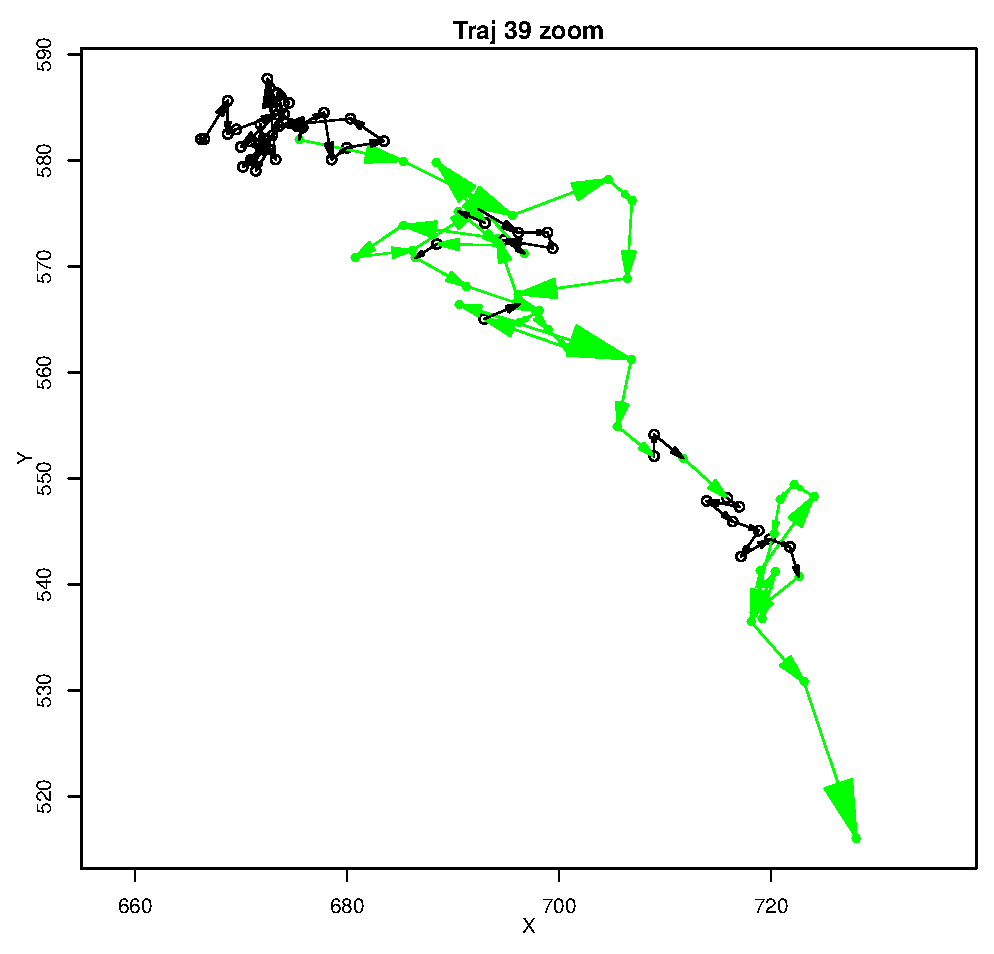
\includegraphics[width=0.5\paperwidth]{track}
            \end{minipage}
            \begin{minipage}{0.5\paperwidth}
                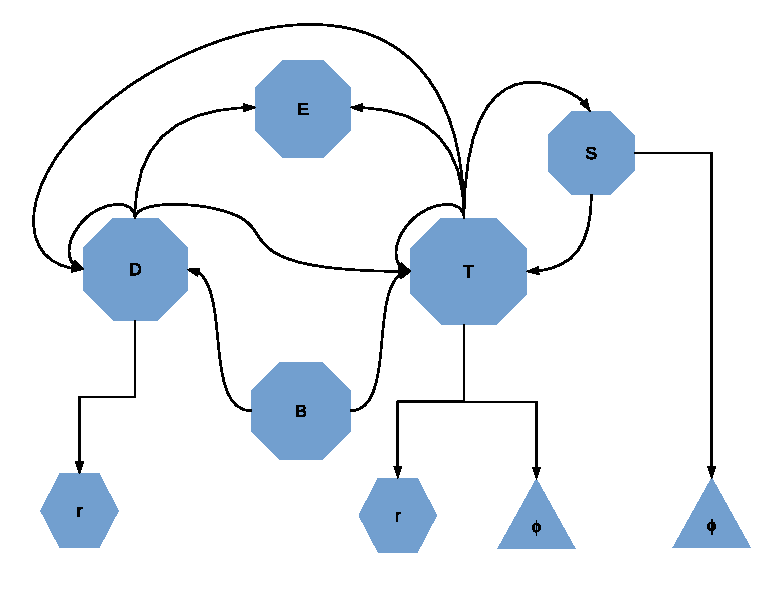
\includegraphics[width=0.5\paperwidth]{hmm}
            \end{minipage}
        }
        \caption{Вероятности переходов СММ между состояниями
        определяются из данных с помощью ППРЭ}
    \end{figure}
\end{frame}

\begin{frame}{Результаты численного эксперимента}
    Проводилось по 100 запусков для каждого набора параметров.
    \begin{figure}
        \makebox[\textwidth]{
            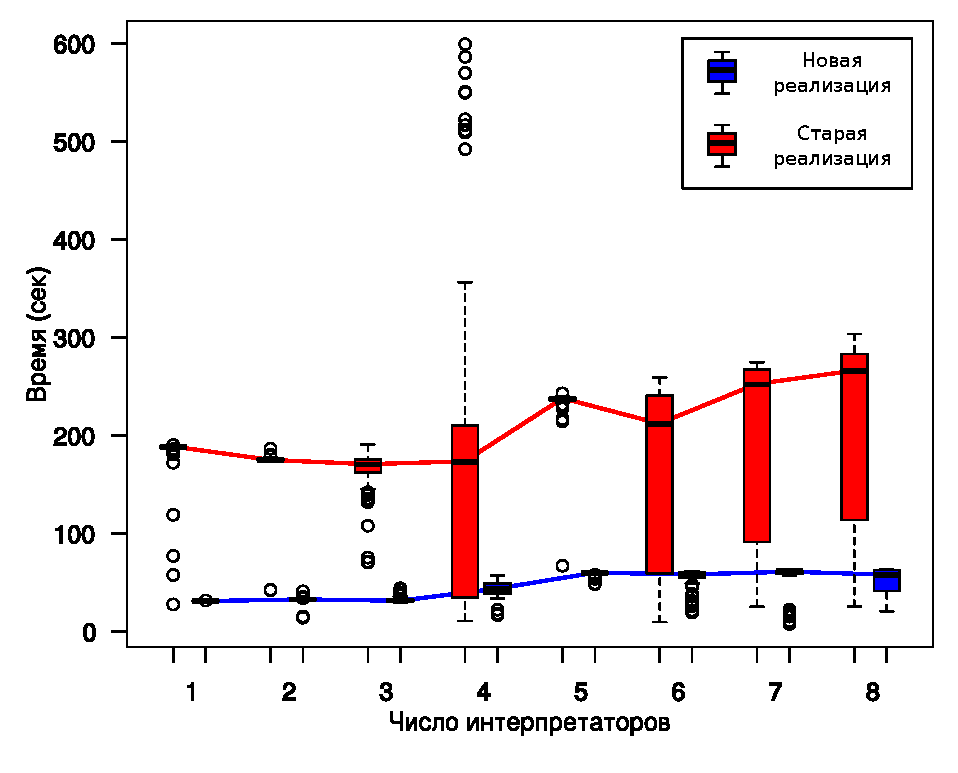
\includegraphics[width=0.5\paperwidth]{m5}
            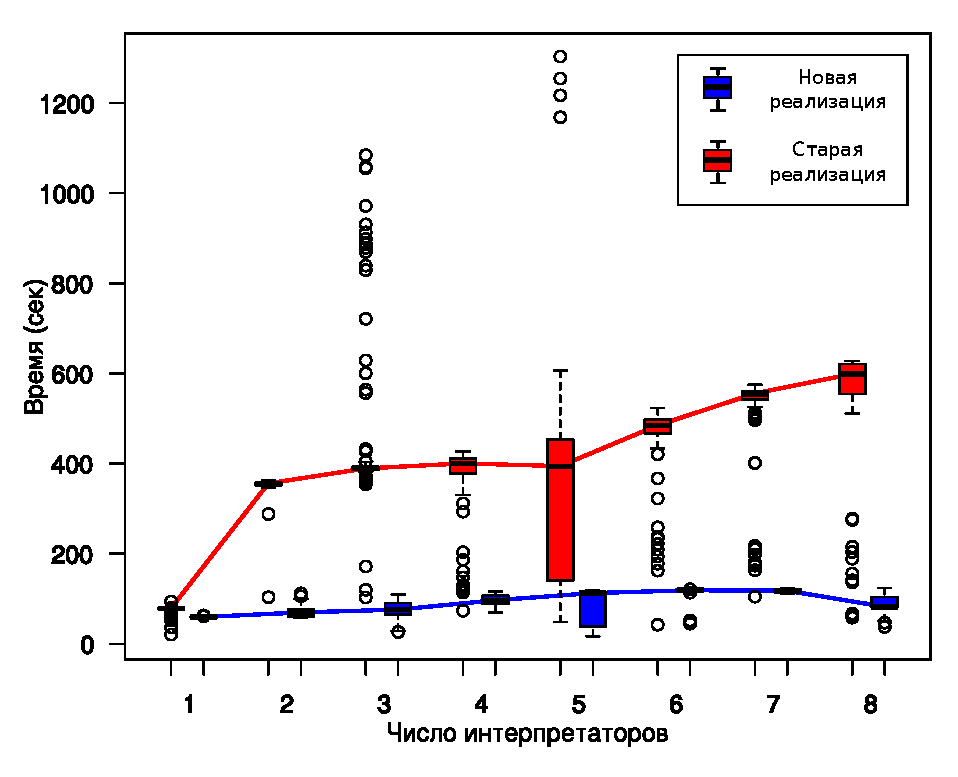
\includegraphics[width=0.5\paperwidth]{m10}
        }
        \caption{Медиана и полтора межквартильных расстояния
            времени выполнения при коэффициенте размера популяции
            5 и 10 соответственно}
    \end{figure}
\end{frame}

\begin{frame}{Критерий Тьюки}
    \textbf{Критерий достоверно значимой разности Тьюки:}
    \bigskip

    Имеется $k$ выборок равного объёма $n$
    из нормально распределённой совокупности:
    \begin{gather*}
        x_{11}, \ldots, x_{1n},\\
        x_{21}, \ldots, x_{2n},\\
        \dots\\
        x_{k1}, \ldots, x_{kn}
    \end{gather*}

    Проверяется гипотеза о статистической неразличимости средних:
    \begin{equation*}
        H_0: \bar{\mu}_1=\bar{\mu}_2=\ldots=\bar{\mu}_k
    \end{equation*}

    Устранение эффекта множественных сравнений:
    \begin{equation*}
        P = 1 - (1 - \alpha)^m \geq \alpha,
    \end{equation*}
    где $\alpha$ вероятность ошибки первого рода.
\end{frame}

\begin{frame}{Статистическая обработка}
    График 95\% доверительных интервалов по критерию Тьюки.
    \begin{columns}
        \begin{column}{0.7\textwidth}
            \begin{figure}[!h]
                \centering
                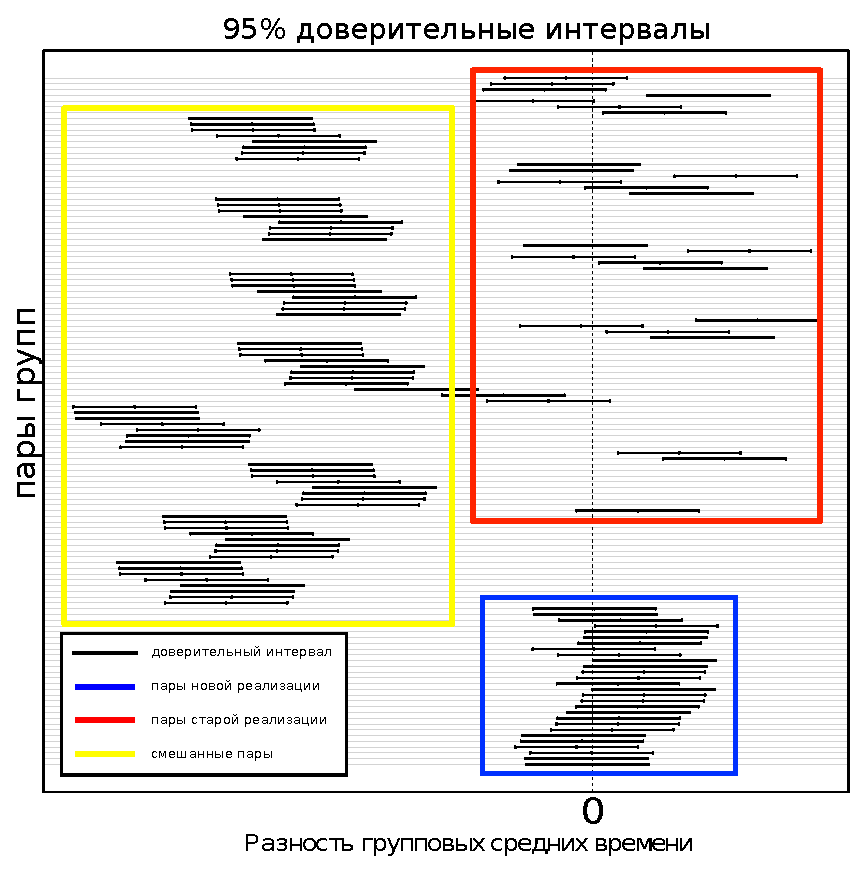
\includegraphics[width=.8\textheight]{tukey}
            \end{figure}
        \end{column}
        \begin{column}{0.4\textwidth}
            \textbf{\textcolor{red}{Красной рамка:}}\\
                старая реализация,
                конкуренция интерпретаторов
                за ресурсы при инициализации;

            \textbf{\textcolor{blue}{Синяя рамка:}}\\
                новая реализация, единичная инициализация;

            \textbf{\textcolor{yellow}{Жёлтая рамка:}}\\
                пары из старой и новой реализаций,
                оптимизация статистически значима.
        \end{column}
    \end{columns}
\end{frame}

\begin{frame}{Выводы}
\begin{itemize}
    \itemsep 2em
    \item Разработанный механизм обеспечивает
        \textbf{4x кратный прирост производительности}
        на 4 параллельных потоках с 4 интерпретаторами по
        сравнению со старой реализацией;
    \item Разработанный механизм \textbf{сохраняет кроссплатформенность} DEEP\\
        (использовалась кроссплатформенная GLib).
\end{itemize}
\end{frame}

\begin{frame}{Благодарности}
    \begin{itemize}
        \itemsep 2em
        \item \textbf{Марии Георгиевне Самсоновой}
        \item \textbf{Константину Николаевичу Козлову}
        \item \textbf{Андрею Сергеевичу Писареву}
    \end{itemize}
    \bigskip

    \vfill
    \begin{center}
        \LARGE Спасибо за внимание!
    \end{center}
\end{frame}

% если не хватит слайда - продолжит на следующих
% t - пытается равномерно распределить
\begin{frame}[t,allowframebreaks]{Используемая литература}
    \nocite{Kozlov11, Kozlov13, Storn95, pisarev2015tracker,
    GLib, zaharie2002parameter, fan2003trigonometric}
    \bibliography{citations}
\end{frame}

\begin{frame}[noframenumbering]{Скрещивание с учётом значения функционала}
    Мутантный вектор:
    \begin{equation*}
        v = v_1 + S \cdot (v_2 - v_3),
    \end{equation*}

    где \begin{math}S\end{math} некоторая положительная константа масштабирования.
    \bigskip

    Второй мутантный вектор:
    \begin{IEEEeqnarray*}{rCl}
        z & = & \frac{v_1 + v_2 + v_3}{3}
        + (s_2 - s_1)(v_1 - v_2) \\
        && + (s_3 - s_2)(v_2 - v_3)
        + (s_1 - s_3)(v_3 - v_1), \nonumber
    \end{IEEEeqnarray*}

    где

    \begin{equation*}
        s_i = \frac{\abs{F(q_i)}}
        {\abs{F(q_1)} + \abs{F(q_2)} + \abs{F(q_3)}},
    \end{equation*}

    для \begin{math}i = 1, 2, 3\end{math}.
\end{frame}

\begin{frame}[noframenumbering]{Скрещивание для поддержания разнообразия индивидов}
    Разнообразие популяции можно определить
    через дисперсии параметров популяции:

    \begin{equation*}
        var_j = \frac{1}{NP} \sum_{i = 0}^{NP - 1}
        \left(q_{i, j} - \frac{1}{NP} \sum_{k = 0}^{NP - 1}q_{k, j}\right)^2
    \end{equation*}
    где $j = 0, \dots, I - 1; I$ --- размер вектора параметров.

    \begin{equation*}
    S_j = \left\{ \,
        \begin{IEEEeqnarraybox}[][c]{l?s}
            \IEEEstrut
            \sqrt{\frac{NP \cdot (c_j - 1) + p_j \cdot (2 - p_j)}
            {2 \cdot NP \cdot p_j}} &
            если $NP \cdot (c_j - 1) + p_j \cdot (2 - p_j) \geq 0$, \\
            S_{inf} & иначе.
            \IEEEstrut
        \end{IEEEeqnarraybox}
        \right.
    \end{equation*}

    где
    \begin{equation*}
        c_j^{new} = \gamma \cdot \left(\frac{var_j}{var_j^{new}}\right)
    \end{equation*}
\end{frame}

\begin{frame}[noframenumbering]{Скрещивание для поддержания разнообразия индивидов}
    \begin{equation*}
    S_j = \left\{ \,
        \begin{IEEEeqnarraybox}[][c]{l?s}
            \IEEEstrut
            \sqrt{\frac{NP \cdot (c_j - 1) + p_j \cdot (2 - p_j)}
            {2 \cdot NP \cdot p_j}} &
            если $NP \cdot (c_j - 1) + p_j \cdot (2 - p_j) \geq 0$, \\
            S_{inf} & иначе.
            \IEEEstrut
        \end{IEEEeqnarraybox}
        \right.
    \end{equation*}

    \begin{equation*}
        p_j = \left\{ \,
            \begin{IEEEeqnarraybox}[][c]{l?s}
                \IEEEstrut
                -(NP \cdot S_j^2 - 1) +
                \sqrt{(NP \cdot S_j^2 - 1)^2 - NP \cdot (1 - c_j)} &
                если $c_j \geq 1$, \\
                p_{inf} & иначе.
                \IEEEstrut
            \end{IEEEeqnarraybox}
            \right.
    \end{equation*}
    где
    \begin{equation*}
        c_j^{new} = \gamma \cdot \left(\frac{var_j}{var_j^{new}}\right)
    \end{equation*}
\end{frame}

\end{document}

